\documentclass[12pt,a4paper]{ctexart}
\usepackage{graphicx}
\usepackage{wrapfig}
\usepackage{float}
\usepackage{siunitx}
\usepackage{subfigure}
\usepackage{caption}
\usepackage{natbib}
\usepackage{listings} % 引入listings宏包用于插入代码
\usepackage{xcolor} % 引入xcolor宏包以支持更多的颜色设置

% 设置Verilog代码样式
\lstdefinestyle{verilog}{
    language=Verilog, % 设置语言为Verilog
    basicstyle=\small\ttfamily, % 设置基本字体样式
    keywordstyle=\color{blue}, % 关键字颜色设置
    commentstyle=\color{gray}\ttfamily, % 注释颜色和样式设置
    stringstyle=\color{red!60!black},
    numbers=left, % 行号在左边显示
    numberstyle=\tiny,
    frame=single, % 添加单线框
    rulecolor=\color{black!30}, % 边框颜色
    breaklines=true, % 允许自动换行
}

\title{实验 2:CPU 功能部件设计}
\author{张子康 \ PB22020660}
\date{2024年04月03日}

\begin{document}
\maketitle
\newpage
\section{实验目的与内容}
\subsection{寄存器堆设计}
设计符合要求的 32 位寄存器堆,并进行仿真。
\subsection{ALU 设计}
设计符合要求的 32 位 ALU,并进行仿真。你需要自行编写合适的仿真文件,验证每一种运算模式下 ALU 计算的正确性。
\subsection{在线计算器}
使用任务 2 中的 ALU,在 FPGAOL 上搭建一个简单的计算器。
\subsection{初始化存储器}
创建一个新的项目,例化合适大小的存储器 IP 核(分布式、块式均可),将上一次实验生成的指令段 COE 文件导入到 IP 核中,并向助教展示。
\section{逻辑设计}
\subsection{寄存器堆设计}
\begin{lstlisting}[style=verilog]
module REG_FILE (
    // 时钟信号
    input [0 : 0] clk, 
    // 寄存器读地址0,五位宽,可选择32个寄存器中的任意一个
    input [4 : 0] rf_ra0, 
    // 寄存器读地址1,同样五位宽,用于第二个读取端口
    input [4 : 0] rf_ra1, 
    // 寄存器写地址,五位宽,指定要写入数据的寄存器位置
    input [4 : 0] rf_wa,
    // 写使能信号,当该信号为高时,允许写操作
    input [0 : 0] rf_we,
    // 数据写入寄存器的数据输入,32位宽
    input [31 : 0] rf_wd,
    // 从寄存器读取的数据输出0,对应ra0指定的寄存器内容
    output [31 : 0] rf_rd0,
    // 从寄存器读取的数据输出1,对应ra1指定的寄存器内容
    output [31 : 0] rf_rd1);

    // 定义一个32x32位的寄存器文件
    // 总共可以存储32个32位的寄存器数据
    reg [31 : 0] reg_file [0 : 31];

    // 用于初始化寄存器
    integer i;
    initial begin
        for (i = 0; i < 32; i = i + 1)
            reg_file[i] = 0;
    end

    // 读取指定寄存器的数据
    assign rf_rd0 = reg_file[rf_ra0];
    assign rf_rd1 = reg_file[rf_ra1];

    // 向指定寄存器写入数据
    always @(posedge clk) begin
        // 指定的寄存器是否为可写入且不是0号寄存器则写入数据
        if (rf_we && rf_wa != 5'd00000)
            reg_file[rf_wa] <= rf_wd;
        else
            reg_file[rf_wa] <= reg_file[rf_wa];
    end

endmodule

\end{lstlisting}
以上代码实现了一个寄存器堆,支持RV32I指令集,具有以下特点:
\begin{enumerate}
    \item 0 号寄存器始终为 0,永远无法被更改;
    \item 
    时钟上升沿到来时,如果写使能信号
    有效,则进行写入操作,否则不进行写入操作;
    \item
    寄存器堆的读操作是时钟异步的(实际上是组
    合逻辑),即只要地址给定,对应寄存器的数值就能读出,
    而无需等待时钟边沿的到来。
\end{enumerate}
\subsection{ALU 设计}
\begin{lstlisting}[style=verilog]
// 定义相应的运算操作码

// 加法
`define ADD                 5'B00000
// 减法
`define SUB                 5'B00010
// 有符号小于
`define SLT                 5'B00100
// 无符号小于
`define SLTU                5'B00101
// 按位与
`define AND                 5'B01001
// 按位或
`define OR                  5'B01010
// 按位异或
`define XOR                 5'B01011
// 左移
`define SLL                 5'B01110
// 逻辑右移
`define SRL                 5'B01111
// 算术右移
`define SRA                 5'B10000
// 选择第一个操作数
`define SRC0                5'B10001
// 选择第二个操作数
`define SRC1                5'B10010

module ALU (input [31 : 0] alu_src0, // 第一个操作数
            input [31 : 0] alu_src1, // 第二个操作数
            input [4 : 0] alu_op,    // 操作码
            output reg [31 : 0] alu_res); // 运算结果

// 内部辅助寄存器,存储操作数的副本,用于计算
reg signed[31:0] tem0;
reg signed[31:0] tem1;

// 时序逻辑块,根据操作码执行相应的运算
always @(*) begin
    tem0 = alu_src0; // 复制第一个操作数
    tem1 = alu_src1; // 复制第二个操作数

    // 根据操作码选择执行哪种运算
    case(alu_op)
        `ADD  : alu_res = tem0 + tem1; // 加法
        `SUB  : alu_res = tem0 - tem1; // 减法
        `SLT  : alu_res = (tem0 < tem1) ? 32'h00000001 : 32'h00000000; // 有符号小于
        `SLTU : alu_res = (alu_src0 < alu_src1) ? 32'h00000001 : 32'h00000000; // 无符号小于
        `AND  : alu_res = tem0 & tem1; // 按位与
        `OR   : alu_res = tem0 | tem1; // 按位或
        `XOR  : alu_res = tem0 ^ tem1; // 按位异或
        `SLL  : alu_res = tem0 << tem1[4:0]; // 左移
        `SRL  : alu_res = tem0 >> tem1[4:0]; // 逻辑右移
        `SRA  : alu_res = tem0 >>> tem1[4:0]; // 算术右移
        `SRC0 : alu_res = alu_src0; // 直接选择第一个操作数
        `SRC1 : alu_res = alu_src1; // 直接选择第二个操作数
        
        // 默认情况下,若操作码不在上述列表中,则将结果清零
        default : alu_res = 32'H0;
    endcase
end

endmodule

\end{lstlisting}
上述代码中定义了一个ALU模块,其中输入为无符号数,tem0与tem1为有符号副本,
回避了一些比较麻烦的手动处理。
\subsection{在线计算器}
\begin{lstlisting}[style=verilog]
module TOP (input [0 : 0] clk,// 时钟信号
    input [0 : 0] rst, // 复位信号
    input [0 : 0] enable, // 写使能信号
    input [4 : 0] in, // 输入信号
    input [1 : 0] ctrl, // 控制信号
    output [3 : 0] seg_data,// 用于驱动七段显示器的数据线
    output [2 : 0] seg_an);// 用于驱动七段显示器的段选线

    // 定义ALU相关信号
    reg [31:0] src0;// 第一个操作数
    reg [31:0] src1;// 第二个操作数
    reg [4:0] op;// 要进行的操作
    wire [31:0] res;// 计算结果
    // 实例化ALU模块
    ALU alu(
        .alu_src0(src0),
        .alu_src1(src1),
        .alu_op(op),
        .alu_res(res)
    );

    // 定义寄存器文件相关的信号
    reg     [ 4 : 0]    ra0, ra1, wa;
    reg     [ 0 : 0]    we;
    reg     [31 : 0]    wd;
    wire    [31 : 0]    rd0;
    wire    [31 : 0]    rd1;
    // 实例化寄存器模块
    REG_FILE regfile (
        .clk    (clk),
        .rf_ra0    (ra0),
        .rf_ra1    (ra1),
        .rf_wa     (wa),
        .rf_we     (we),
        .rf_wd     (wd),
        .rf_rd0    (rd0),
        .rf_rd1    (rd1)
    );

    // 实例化Segment模块
    Segment segment(
        .clk(clk),
        .rst(rst),
        .output_data(res),
        .seg_data(seg_data),
        .seg_an(seg_an)
    );

    // flage用于确定当前是否进行计算
    reg flage;
    // t0和t1用于进行计数,确定当前进行的步骤
    reg [2:0] t0;
    reg [2:0] t1;

    // 初始化
    initial begin
        src0=0;
        src1=0;
        op=0;
        ra0=0;
        ra1=0;
        wa=0;
        we=1'b1;
        wd=0;
        flage=0;
        t0=0;
        t1=0;
    end

    always @(posedge clk) begin
        // 处理复位信号,不对寄存器进行操作
        if(rst)begin
            src0<=0;
            src1<=0;
            op<=0;
            ra0<=0;
            ra1<=0;
            wa<=0;
            we<=1'b1;
            wd<=0;
            flage<=0;
            t0<=0;
            t1<=0;
        end else begin
            // 判断当前是否需要从寄存器读取数据进行操作
            if(flage) begin
                // 先从寄存器读取op和第一个操作数
                if(t0==3'h0) begin
                    op<=rd0[4:0];
                    src0<=rd1;
                    t1<=t0+1;
                    t0<=t1+1;
                end else begin
                    // 将读取的寄存器地址指向第二个操作数所在的寄存器
                    if(t0==3'h1) begin
                        ra1<=5'h3;
                        t0<=t1+1;
                        t1<=t0+1;
                    end else begin
                    // 读取第二个操作数并将flage,t0和t1值复位
                        src1<=rd1;
                        t0<=0;
                        t1<=0;
                        flage<=0;
                    end
                end
            end else begin
                // 判断当前是否按下按钮,如果按下就储存当前数据
                if(enable)
                    // 判断当前要进行的操作
                    case(ctrl)
                        // 输入OP,进行无符号扩展
                        2'b00:
                        begin 
                            wd<={27'h0,in};
                            wa<=5'h1;
                        end
                        // 输入第一个操作数,并进行符号扩展
                        2'b01:
                        begin 
                            wd<={{27{in[4]}},in};
                            wa<=5'h2;
                        end
                        // 输入第二个操作数,并进行符号扩展
                        2'b10:
                        begin
                            wd<={{27{in[4]}},in};
                            wa<=5'h3;
                        end
                        // 进行计算
                        2'b11:
                        begin
                            ra0<=5'h1;
                            ra1<=5'h2;
                            flage<=1;
                            t0<=0;
                            t1<=0;
                        end
                    endcase
                else begin
                    src0<=src0;
                    src1<=src1;
                    op<=op;
                    ra0<=ra0;
                    ra1<=ra1;
                    wa<=wa;
                    we<=1'b1;
                    wd<=wd;
                end
            end
        end
    end
endmodule

\end{lstlisting}
以上为计算器的TOP模块。\par
实际上本题并未要求使用寄存器堆,以上代码实现的过于麻烦了。
可以直接利用op,src0与src1进行存储,以此可以极大的简化代码。
\subsection{初始化存储器}
例化合适大小的分布式存储器 IP 核
,将上一次实验生成的指令段 COE 文件导入到 IP 核中。
图片如下:
\begin{center}
    \begin{figure}[h]
        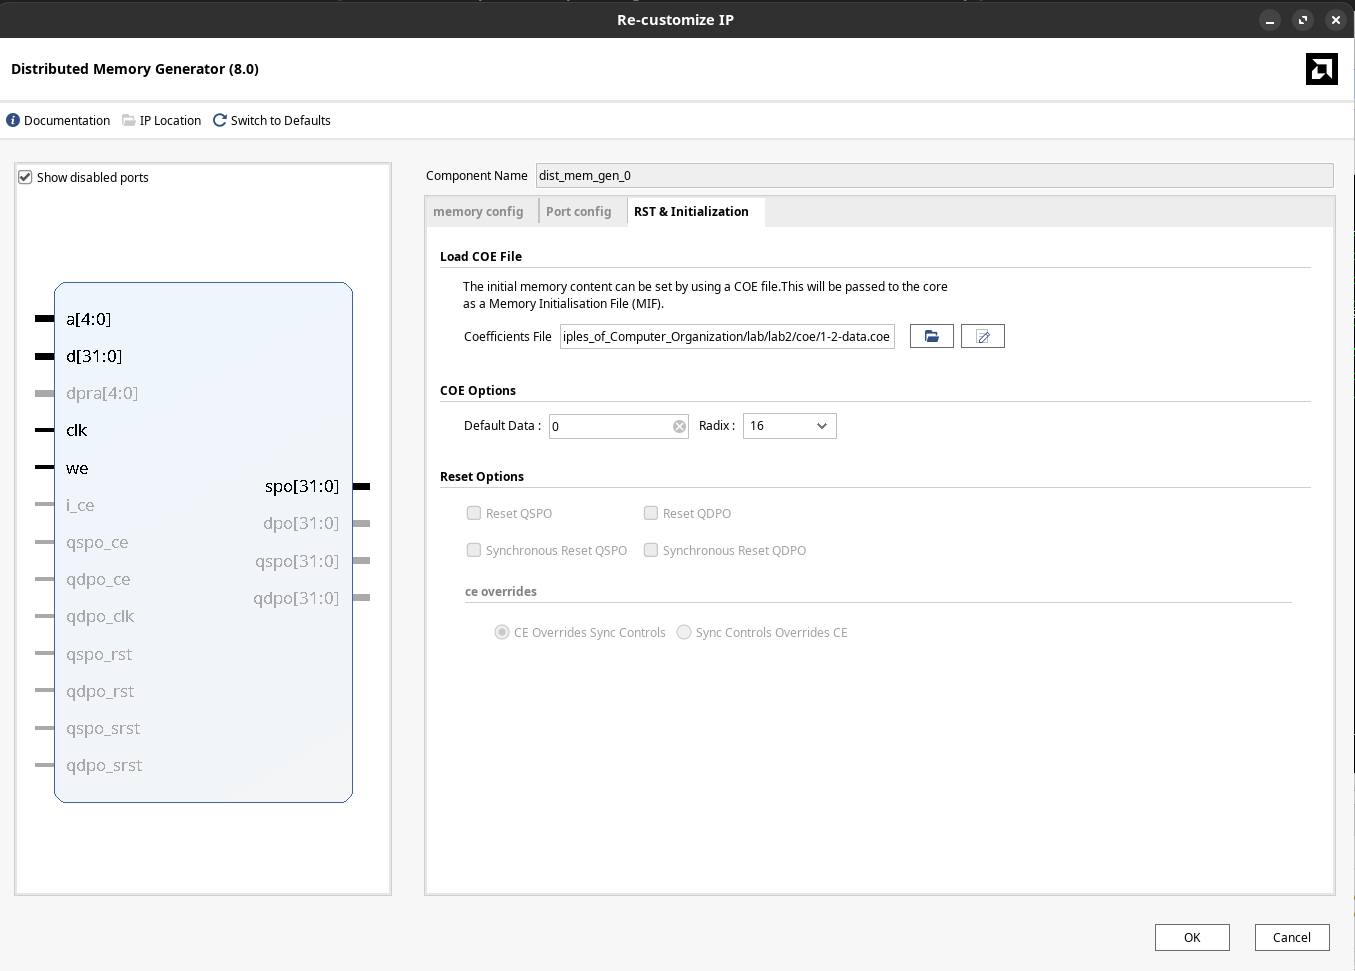
\includegraphics[scale=0.38]{pic/2024-04-03_23-48.png}
        \caption{导入的coe文件}
    \end{figure}
\end{center}
\section{仿真结果与分析}
\subsection{寄存器堆设计}
仿真代码如下:
\begin{lstlisting}[style=verilog]
module RegFile_tb ();
    reg                 clk;
    reg     [ 4 : 0]    ra0, ra1, wa;
    reg     [ 0 : 0]    we;
    reg     [31 : 0]    wd;
    wire    [31 : 0]    rd0;
    wire    [31 : 0]    rd1;

    REG_FILE regfile (
        .clk    (clk),
        .rf_ra0    (ra0),
        .rf_ra1    (ra1),
        .rf_wa     (wa),
        .rf_we     (we),
        .rf_wd     (wd),
        .rf_rd0    (rd0),
        .rf_rd1    (rd1)
    );

    initial begin
        clk = 0;
        ra0 = 5'H0; ra1 = 5'H0; wa = 5'H0; we = 1'H0; wd = 32'H0;

        #12
        ra0 = 5'H0; ra1 = 5'H0; wa = 5'H3; we = 1'H1; wd = 32'H12345678;

        #5
        ra0 = 5'H0; ra1 = 5'H0; wa = 5'H0; we = 1'H0; wd = 32'H0;

        #5
        ra0 = 5'H3; ra1 = 5'H2; wa = 5'H2; we = 1'H1; wd = 32'H87654321;

        #5
        ra0 = 5'H0; ra1 = 5'H0; wa = 5'H0; we = 1'H0; wd = 32'H0;

        #5
        ra0 = 5'H3; ra1 = 5'H0; wa = 5'H0; we = 1'H1; wd = 32'H87654321;

        #10
        $finish;
    end
    always #5 clk = ~clk;
endmodule
\end{lstlisting}
仿真结果如图:
\begin{center}
    \begin{figure}[ht]
        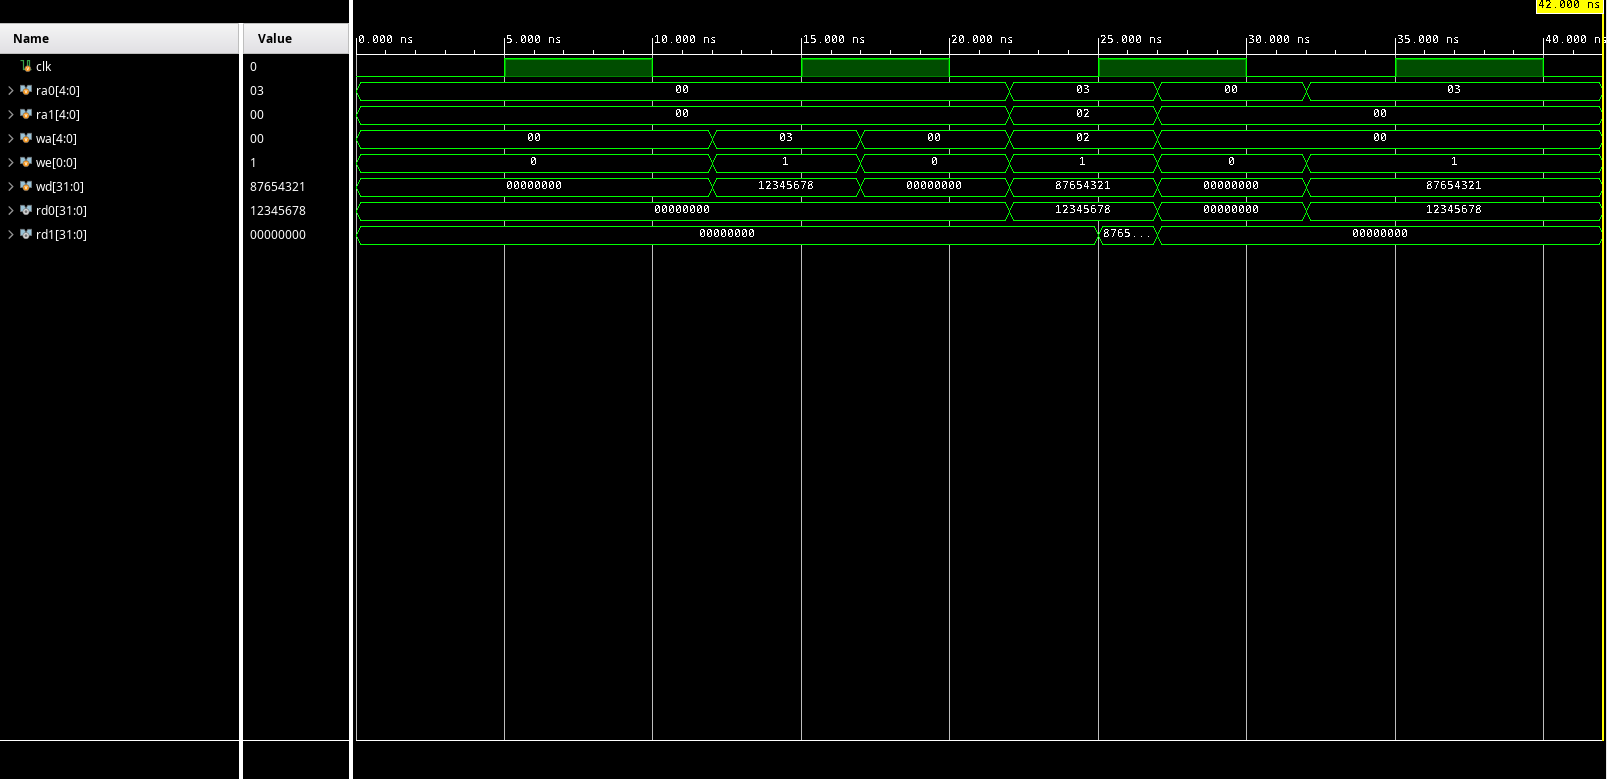
\includegraphics[scale=0.35]{pic/2024-04-03_23-55.png}
        \caption{寄存器堆仿真结果}
    \end{figure}
\end{center}
\newpage
\subsection{ALU 模块}
仿真代码如下:
\begin{lstlisting}[style=verilog]
`timescale 1ns / 1ps
module alu_testbench();
    parameter clk_sep  = 1;
    parameter time_sep = 10;
    reg [31:0] src0;
    reg [31:0] src1;
    reg [4:0] op;
    wire [31:0] res;
    reg clk;
    ALU alu(
        .alu_src0(src0),
        .alu_src1(src1),
        .alu_op(op),
        .alu_res(res)
    );
    initial begin
        clk=0;
        forever begin
            #time_sep
            clk=~clk;
        end
    end
    initial begin
        src0=32'h81111111;
        src1=32'h11111111;
        op=5'B00000;
        #clk_sep
        op=5'B00010;
        #clk_sep
        op=5'B00100;
        #clk_sep
        op=5'B00101;
        #clk_sep
        op=5'B01001;
        #clk_sep
        op=5'B01010;
        #clk_sep
        op=5'B01011;
        #clk_sep
        op=5'B01110;
        #clk_sep
        op=5'B01111;
        #clk_sep
        op=5'B10000;
        #clk_sep
        op=5'B10001;
        #clk_sep
        op=5'B10010;
        #clk_sep
        $finish;
    end
endmodule
\end{lstlisting}
仿真结果如图:
\begin{center}
    \begin{figure}[ht]
        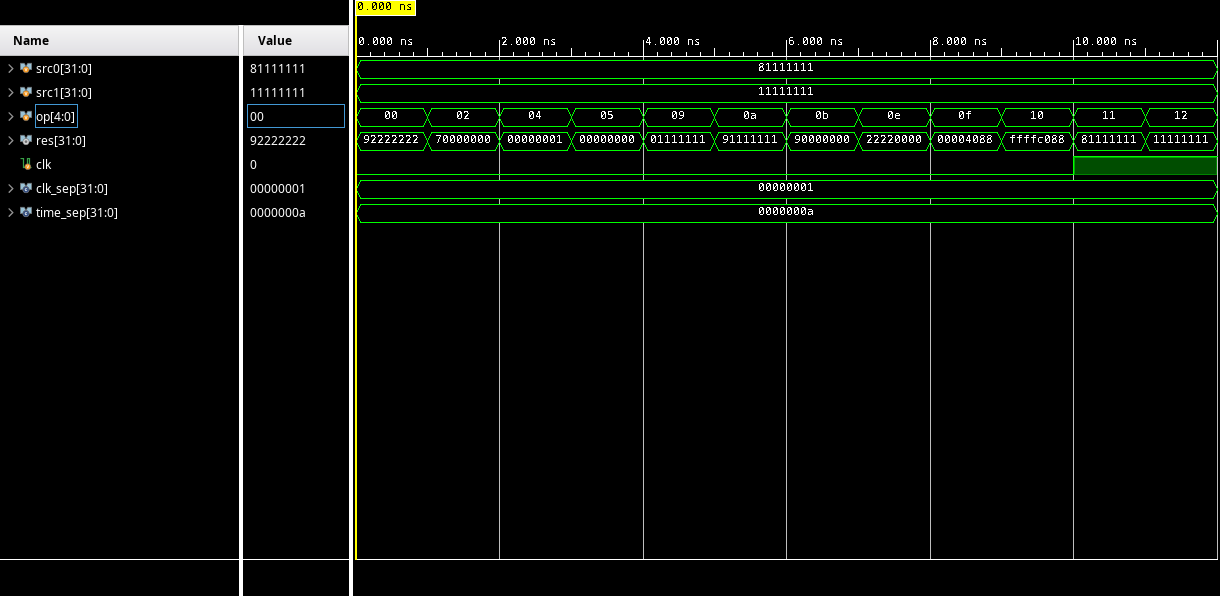
\includegraphics[scale=0.5]{pic/2024-04-03_23-53.png}
        \caption{ALU模块仿真结果}
    \end{figure}
\end{center}
\section{电路设计与分析}
\newpage
\begin{center}
    \begin{figure}[t]
        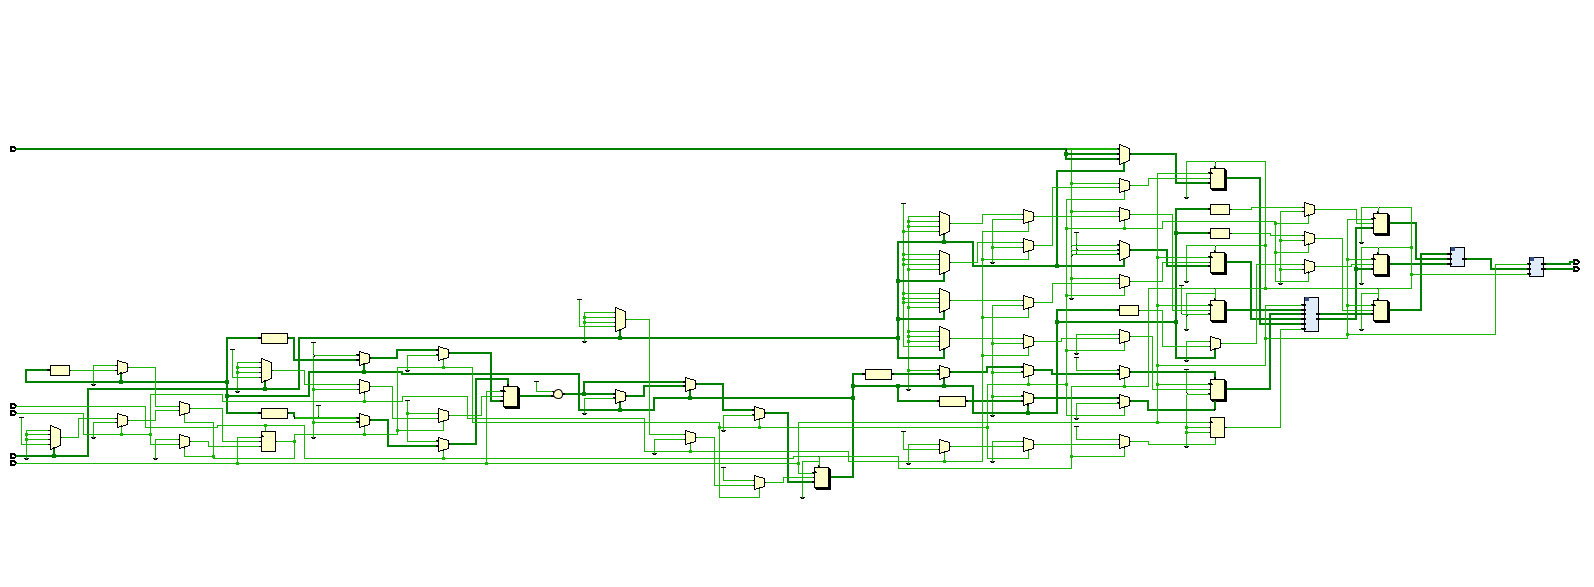
\includegraphics[scale=0.4]{pic/2024-04-04_00-08.png}
        \caption{完整的电路图}
    \end{figure}
\end{center}
\section{测试结果与分析}
\subsection{在线计算器}
将编译好的bit文件导入FPAGOL,并且输入
$OP=5'b00010,SRC0=5'b00001,SRC1=5'b111111$,计算结果如图所示:
\newpage
\begin{center}
    \begin{figure}[t]
        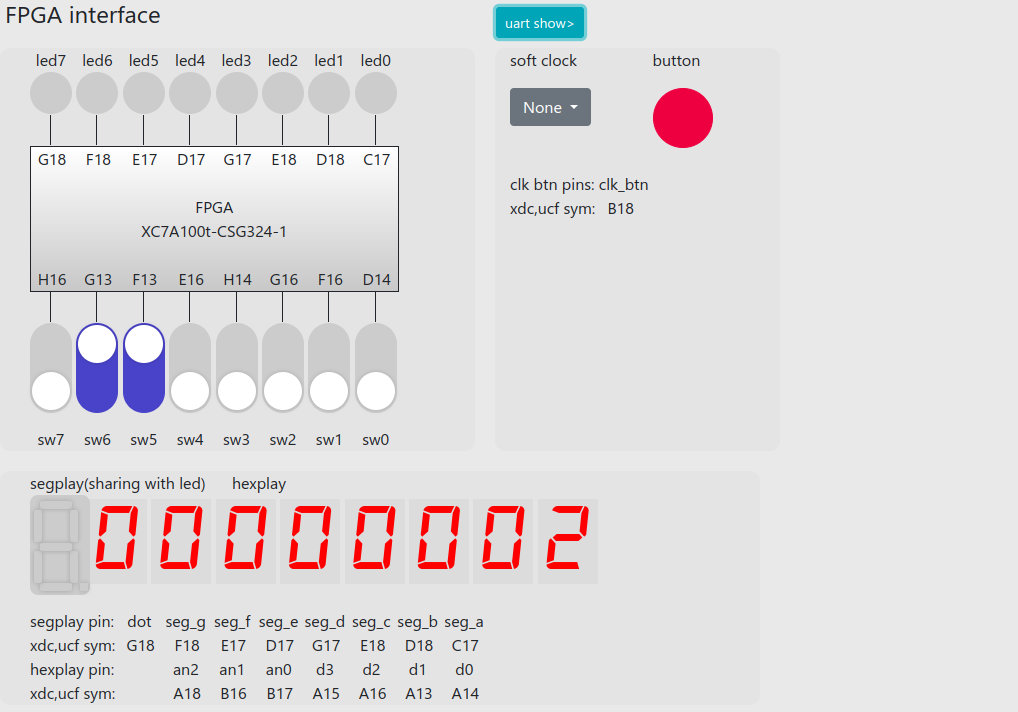
\includegraphics[scale=0.5]{pic/2024-04-04_00-00.png}
        \caption{FPAG运行结果}
    \end{figure}
\end{center}
\section{总结}
通过本次实验初步掌握了verilog,并完成了寄存器堆、ALU模块、在线计算器的设计
与ip核初始化。
\end{document}